	%-=-=-=-=-=-=-=-=-=-=-=-=-=-=-=-=-=-=-=-=-=-=-=-=
%
%        LOADING DOCUMENT
%
%-=-=-=-=-=-=-=-=-=-=-=-=-=-=-=-=-=-=-=-=-=-=-=-=

\documentclass[newPxFont,pagenumber]{beamer}
\usetheme{sthlm}
%\usecolortheme{sthlmv42}

%-=-=-=-=-=-=-=-=-=-=-=-=-=-=-=-=-=-=-=-=-=-=-=-=
%        LOADING PACKAGES
%-=-=-=-=-=-=-=-=-=-=-=-=-=-=-=-=-=-=-=-=-=-=-=-=
\usepackage[utf8]{inputenc}
\usepackage[frenchb]{babel}
\usepackage[normalem]{ulem}
\usepackage{caption}
\captionsetup{font=scriptsize}
%\usepackage[font=footnotesize]{subcaption}
% in preamble
\usepackage{chronology}
\usepackage{pgf}
\usepackage{tikz}
\usetikzlibrary{arrows,automata}

\usepackage{nameref}
\makeatletter
\newcommand*{\currentname}{\@currentlabelname}
\makeatother

\graphicspath{ {fig/} }

\usepackage[linesnumbered,ruled,vlined]{algorithm2e}
% add page number
%\usepackage[defaultsans]{cantarell}

\newcommand{\p}{\mathbb{P}}

\setbeamerfont{title}{series=\upshape}
\setbeamertemplate{footline}{\hfill\footnotesize\insertframenumber\hskip3pt\null\vskip3pt}

\newcommand{\argmax}{\mathop{\mathrm{argmax}}\limits}
\renewcommand{\max}{\mathop{\mathrm{max}}\limits}

\renewcommand{\event}[3][e]{%
  \pgfmathsetlength\xstop{(#2-\theyearstart)*\unit}%
  \ifx #1e%
    \draw[fill=black,draw=none,opacity=0.5]%
      (\xstop, 0) circle (.2\unit)%
      node[opacity=1,rotate=45,right=.2\unit] {#3};%
  \else%
    \pgfmathsetlength\xstart{(#1-\theyearstart)*\unit}%
    \draw[fill=black,draw=none,opacity=0.5,rounded corners=.1\unit]%
      (\xstart,-.1\unit) rectangle%
      node[opacity=1,rotate=45,right=.2\unit] {#3} (\xstop,.1\unit);%
  \fi}%

\addto\captionsfrench{%
\renewcommand{\figurename}{\scriptsize {\scshape Figure}}
\renewcommand{\tablename}{\scriptsize {\scshape Table}}
}

%-=-=-=-=-=-=-=-=-=-=-=-=-=-=-=-=-=-=-=-=-=-=-=-=
%        BEAMER OPTIONS
%-=-=-=-=-=-=-=-=-=-=-=-=-=-=-=-=-=-=-=-=-=-=-=-=

%\setbeameroption{show notes}

%-=-=-=-=-=-=-=-=-=-=-=-=-=-=-=-=-=-=-=-=-=-=-=-=
%
%	PRESENTATION INFORMATION
%
%-=-=-=-=-=-=-=-=-=-=-=-=-=-=-=-=-=-=-=-=-=-=-=-=

\title{\normalsize Analyse Sémantique d'un Corpus Exhaustif de Décisions Jurisprudentielles pour l'Élaboration d'un Modèle Prédictif du Risque Judiciaire}
\subtitle{\small Séminaire e-juris
%\includegraphics[width=0.15\paperwidth]{ProfitLossRiskDecisionOutcomeLg.png}
}
%\date{\small{\jobname}}
%\date{\today}
\date{\scriptsize 24 mars 2017}
\author{\textbf{TAGNY NGOMPE Gildas\textsuperscript{\ref{lgi2p},\ref{chrome}}}, Sébastien Harispe\textsuperscript{\ref{lgi2p}}, Jacky Montmain\textsuperscript{\ref{lgi2p}}, Stéphane Mussard\textsuperscript{\ref{chrome}}, Guillaume Zambrano\textsuperscript{\ref{chrome}}}
%\institute{\small\textbf{Directeur}: Stéphane Mussard, Pr. (CHROME, Univ. Nîmes)  \\ \textbf{Co-directeur}: Jacky Montmain, Pr. (LGI2P, Ecole des Mines d'alès) \\ \textbf{Encadrants}: Guillaume Zambrano, Sébastien Harispe}
\institute{%\scriptsize  
\begin{enumerate}
\item LGI2P (École des mines d'Alès) \label{lgi2p}
\item CHROME EA 7352 (Université de Nîmes) \label{chrome}
\end{enumerate}
}

\hypersetup{
pdfauthor = {\author{}: tagnyngompe@gmail.com},
pdfsubject = {},
pdfkeywords = {},
pdfmoddate= {D:\pdfdate},
pdfcreator = {}
}

\begin{document}
\nocite{}
%-=-=-=-=-=-=-=-=-=-=-=-=-=-=-=-=-=-=-=-=-=-=-=-=
%
%	TITLE PAGE
%
%-=-=-=-=-=-=-=-=-=-=-=-=-=-=-=-=-=-=-=-=-=-=-=-=
\begin{frame}[plain]
	\titlepage
\end{frame}
%}
%-=-=-=-=-=-=-=-=-=-=-=-=-=-=-=-=-=-=-=-=-=-=-=-=
%
%	TABLE OF CONTENTS: Plan
%
%-=-=-=-=-=-=-=-=-=-=-=-=-=-=-=-=-=-=-=-=-=-=-=-=
\section*{Plan}
\begin{frame}[c]{\currentname}
\tableofcontents[hideallsubsections]
\end{frame}
%-=-=-=-=-=-=-=-=-=-=-=-=-=-=-=-=-=-=-=-=-=-=-=-=
%
%	Section: Positionnement
%
%-=-=-=-=-=-=-=-=-=-=-=-=-=-=-=-=-=-=-=-=-=-=-=-=
\section{Motivations et problématiques}
\begin{frame}[c]{Thèse de doctorat}
\Large\textbf{Analyse Sémantique d'un Corpus Exhaustif} de \textbf{Décisions
Jurisprudentielles} pour l'Élaboration d'un \textbf{Modèle Prédictif du
Risque} Judiciaire

\vspace{0.4cm}

\hfill
\includegraphics[scale=0.25]{ED583.jpg}
\end{frame}

\begin{frame}[c]{Les juristes analysent les décisions afin d'anticiper}
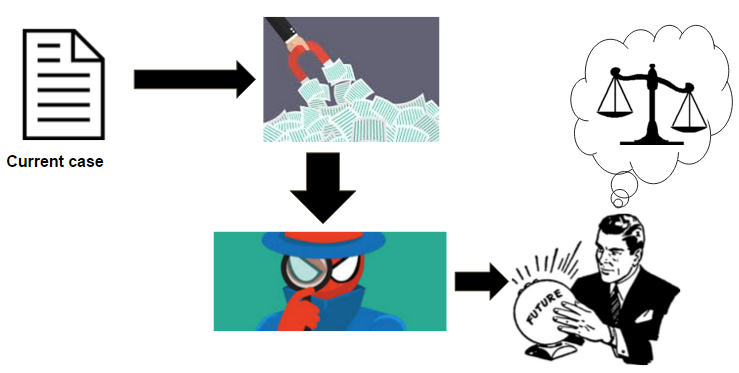
\includegraphics[width=\textwidth]{lawyerwork.PNG}
\end{frame}

\begin{frame}{Défis liés à la recherche et à l'analyse}
\begin{itemize}
\item Grande quantité des décisions
\item Documents non-structurés
\item Complexité de l'organisation de la justice 
\item Compréhension difficile du langage juridique
\end{itemize}
\end{frame}

\begin{frame}{Objectif: un pipeline d'analyse de corpus jurisprudentiels}
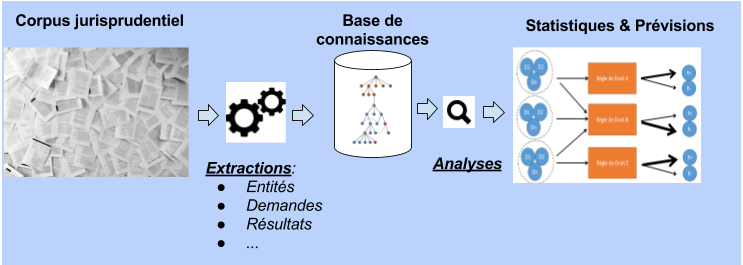
\includegraphics[width=\textwidth]{pipeline-cassandra.png}
\end{frame}

\begin{frame}{Informations pertinentes à extraire}
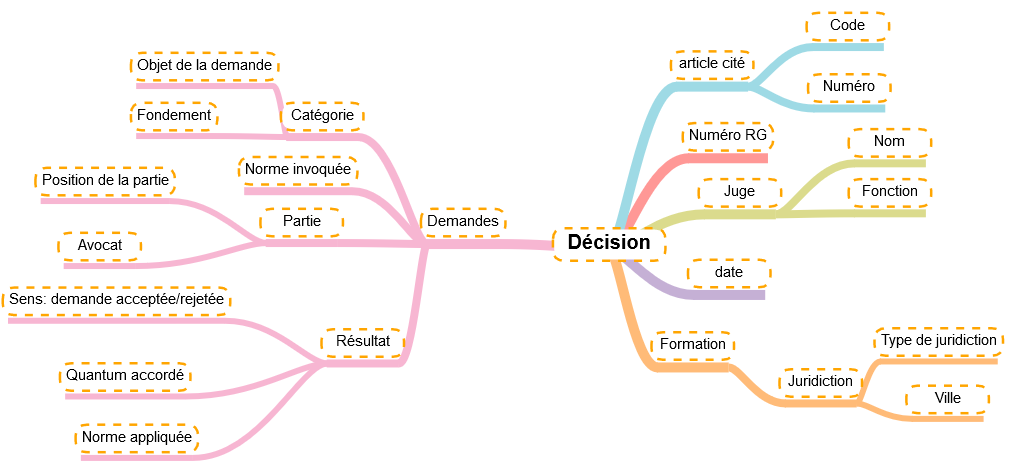
\includegraphics[width=0.9\paperwidth]{arbre-des-infos.PNG}

%\textbf{Problématiques:}
%\begin{itemize}
%\item Extraction et résolution des méta-données 
%\item Extraction des demandes et de leur résultat
%\item 
%\end{itemize}

\end{frame}

\begin{frame}{Structure dans la base de connaissances}
\begin{figure}
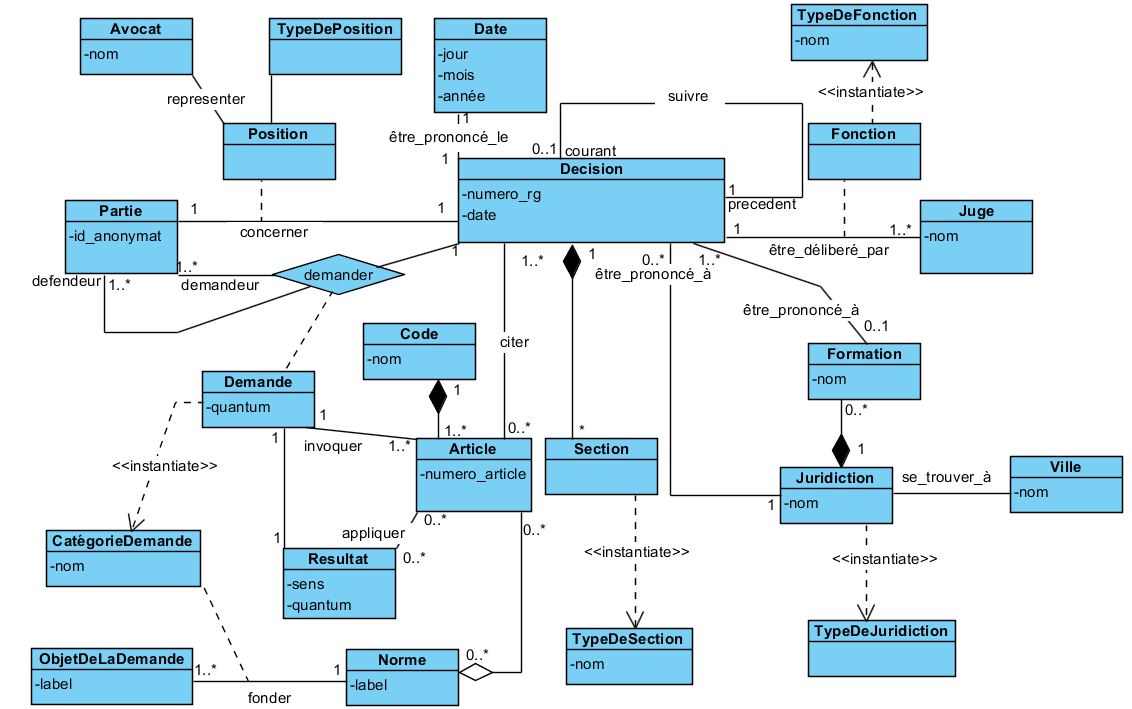
\includegraphics[width=0.8\paperwidth]{class-diagram.png}
\caption{Modèle des données}
\end{figure}
\end{frame}


%-=-=-=-=-=-=-=-=-=-=-=-=-=-=-=-=-=-=-=-=-=-=-=-=
%
%	Section: Extraction d'information à partir de décisions
%
%-=-=-=-=-=-=-=-=-=-=-=-=-=-=-=-=-=-=-=-=-=-=-=-=
\section{Segmentation et détection d'entités}

\begin{frame}{Informations noyées dans des textes non-structurées}
\scriptsize
\begin{columns}
\begin{column}{.50\linewidth}
ARRÊT N°

R.G: 11/03924

...

{COUR D'APPEL} DE {NÎMES}

{CHAMBRE CIVILE}

{1ère Chambre A}

ARRÊT DU {20 MARS 2012}

APPELANTE:

{Madame Michéle A.} ...

assistée de la {SELARL VAJOU}, ...

INTIMES:

{Monsieur Martial B} ...

assisté de la {SCP MARION GUIZARD PATRICIA SERVAIS}, ...

COMPOSITION DE LA COUR LORS DU DÉLIBÉRÉ:

{M. Dominique BRUZY, Président}

{M. Serge BERTHET, Conseiller}

...
\end{column}
\begin{column}{.50\linewidth}
FAITS, PROCEDURE, ...

Madame Michèle A. demande:

...

- de condamner Madame JONES-B. à lui payer la somme de {2.500 euros} au titre de l'{article 700 du Code de Procédure Civile}, 

\vspace{0.4cm}

PAR CES MOTIFS, LA COUR:

...

Vu l'{article 809 du Code de Procédure Civile},

...

{Déboute Madame A. de sa demande de provision sur dommages-intérêts.}

...

Vu l'{article 700 du Code de Procédure Civile},

Condamne Madame JONES-B. à verser à Madame A. la somme de {2.500 euros}.
\end{column}
\end{columns}
\end{frame}

\begin{frame}{Sectionner les décisions pour organiser l'extraction}
\scriptsize
\begin{columns}
\begin{column}{.45\linewidth}
\fbox{\begin{minipage}{\textwidth}ARRÊT N°

R.G: \textcolor{red}{11/03924}

\textcolor{red}{COUR D'APPEL} DE \textcolor{red}{NÎMES}

\textcolor{red}{CHAMBRE CIVILE}

\textcolor{red}{1ère Chambre A}

ARRÊT DU \textcolor{red}{20 MARS 2012}

APPELANTE:

\textcolor{red}{Madame Michéle A.} ...

assistée de la \textcolor{red}{SELARL VAJOU}, ...

INTIMES:

\textcolor{red}{Monsieur Martial B} ...

assisté de la \textcolor{red}{SCP MARION GUIZARD PATRICIA SERVAIS}, ...

COMPOSITION DE LA COUR LORS DU DÉLIBÉRÉ:

\textcolor{red}{M. Dominique BRUZY, Président}

\textcolor{red}{M. Serge BERTHET, Conseiller}

...
\end{minipage}}
\vspace{0.1cm}

{\normalsize \textbf{Entêtes}: méta-données}
\end{column}
\begin{column}{.55\linewidth}
\fbox{\begin{minipage}{\textwidth}FAITS, PROCEDURE, ...

Madame Michèle A. demande:

...

- de condamner Madame JONES-B. à lui payer la somme de \textcolor{red}{2.500 euros} au titre de l'\textcolor{red}{article 700 du Code de Procédure Civile}, 
\end{minipage}}
\vspace{0.1cm}

{\normalsize \textbf{Corps}: demandes et normes }

\vspace{0.4cm}

\fbox{\begin{minipage}{\textwidth}PAR CES MOTIFS, LA COUR:

...

Vu l'\textcolor{red}{article 809 du Code de Procédure Civile},

...

\textcolor{red}{Déboute Madame A. de sa demande de provision sur dommages-intérêts.}

...

Vu l'\textcolor{red}{article 700 du Code de Procédure Civile},

Condamne Madame JONES-B. à verser à Madame A. la somme de \textcolor{red}{2.500 euros}.
\end{minipage}}
\vspace{0.1cm}

{\normalsize \textbf{Dispositif}: résultats et normes}

\end{column}
\end{columns}
\end{frame}

\begin{frame}{Entités et sections à détecter}

\scriptsize
\begin{table}[!htb]
\centering
%\scriptsize
\begin{tabular}[c]{|l|c|p{0.6\textwidth}|}
\hline
\textbf{Entités} & \textbf{Labels} & \textbf{Exemples}\\\hline
\multicolumn{3}{|c|}{\textbf{Section entête (E)}} \\
\hline
Numéro R.G. & \textbf{RG} & "10/02324", "60/JAF/09" \\ \hline
Ville & \textbf{VL}& "NÎMES", "Agen", "Toulouse" \\ \hline
Type de juridiction & \textbf{JR} & "COUR D'APPEL" \\ \hline
Formation & \textbf{FM} & "1re chambre", "Chambre économique" \\ \hline
Date & \textbf{DT} & "01 MARS 2012", "15/04/2014"\\ \hline
Partie appelante & \textbf{AP} & "SARL K.", "Syndicat ...", "Mme X ..."\\ \hline
Partie intimée & \textbf{IM} & - // - \\ \hline
Partie intervenante & \textbf{IV} & - // - \\ \hline
Avocat & \textbf{AV} & "Me Dominique A., avocat au barreau de Papeete"\\ \hline
Juge & \textbf{JG} & "Monsieur André R.", "Mme BOUSQUEL" \\ \hline
fonction du juge & \textbf{FT} & "Conseiller", "Président"\\ \hline
\multicolumn{3}{|c|}{\textbf{Corps (T) et dispositif (D)}} \\ \hline

Norme & \textbf{NO} & "l' article 700 NCPC", "articles 901 et 903"  \\ \hline
\hline
Élément à éviter & \textbf{O} & \textit{tout élément ne faisant partie d'aucune entité ciblée} \\ \hline
\end{tabular} 

\caption{Entités et leurs labels par section.}\label{relevantinfo}
\end{table}
\end{frame}

\begin{frame}{Approches probabilistes d'étiquetage de séquence}
Modèles probabilistes à états et observations

\scriptsize
\begin{table}[]%width=\linewidth
	%\begin{tabular}[]{p{0.40\linewidth}|p{0.55\linewidth}}
	\begin{tabular}[]{c|c}
		\toprule
{\textbf{HMM}} & {\textbf{CRF}} \\
%		\midrule
%		\textbf{Generative} models 	& \multicolumn{2}{c}{"\textbf{Discriminative}" or "\textbf{Conditional}" models } \\[0.25em]
%\midrule		
%"\textbf{generate}" input	& {"\textbf{condition}" on input }\\%[0.25em]
\midrule
{un seul descripteur  par observation}	& {plusieurs descripteurs complexes par observation}\\%[0.25em]
\midrule	
		\begin{tikzpicture}[->,>=stealth',shorten >=1pt,auto,node distance=1.3cm,
                    semithick]
  \node[state] (S1)                    {$s_{t-1}$};
  \node[state]         (S2) [right of=S1] 	  {$s_{t}$};
  \node[state]         (O) [below of=S2] {$o_{t}$};
  \path (S1) edge              node {} (S2)
        (S2) edge              node {} (O);
\end{tikzpicture}
				& 

\begin{tikzpicture}[auto,>=stealth',shorten >=1pt,auto,node distance=1.3cm,
                    semithick]
  \node[state] (S1)                    {$s_{t-1}$};
  \node[state]         (S2) [right of=S1] 	  {$s_{t}$};
  \node[state]         (O) [below of=S2] {$o_{t}$};
  \path (S1) edge              node {} (S2)
        (S2) edge              node {} (O);
\end{tikzpicture}					
					\\%[0.25em]
\midrule
$P_\lambda(S|O) = \prod\limits_{t=1}^{T} P(s_t \vert s_{t-1}) * P(o_t \vert s_{t})$  & $P_\lambda(S|O) = \frac{1}{Z(O)}exp\left( \sum\limits_{t=1}^{T}\sum\limits_{k} \lambda_k f_k(s_{t-1},s_t, o_t) \right) $ \\
% & & & \\
\tiny \cite{Seymore1999hmm} & \tiny \cite{peng2006crf} \\ 
		\bottomrule
	\end{tabular}
\end{table}

\normalsize

Objectif: Trouver la séquence la plus probable d'étiquetage pour l'ensemble du texte

\textbf{Entrainement fait sur des séquences préalablement étiquetées}
\end{frame}

\begin{frame}[c]{Introduire des descripteurs discriminants dans les modèles}
Exemple : Soit l'annotation manuelle : 

\og \textit{... l' @NO article 700 du code de procédure \#NO ...} \fg{}

Introduction des caractéristiques au niveau de $t_i$ = \og 700 \fg{}
\footnotesize


\[f_1(l_{i-1},l_i,t_{1:n},i) = \left\lbrace \begin{array}{ll}
b_1(T,i) & \text{si } l_{i-1} = \text{NORME} \wedge l_i = \text{NORME} \\
0 & \text{sinon}
\end{array} \right.\]
\[f_2(l_{i-1},l_i,t_{1:n},i) = \left\lbrace \begin{array}{ll}
b_2(T,i) & \text{si }l_i = \text{NORME} \\
0 & \text{sinon}
\end{array} \right.\]
avec 
\[b_1(T,i) = \left\lbrace \begin{array}{ll}
1 & \text{si } (t_{i-1} =\text{article) }\wedge (POS_{i-1}=\text{NOM}) \\ &  \wedge  (NP1_{i-1}=\text{<unknown>)} \wedge (NS1_{i-1}=\text{@card@)} \\
0 & \text{sinon} 
\end{array} \right.\]
\[b_2(T,i) = \left\lbrace \begin{array}{ll}
1 & \text{si } (t_i =\text{700) }\wedge (POS_i=\text{NUM})  \wedge (NP1_i=\text{article)} \wedge (NS1_i=\text{code)} \\
0 & \text{sinon}
\end{array} \right.\]

\cite{Wallach2004crfintro}
\end{frame}


\begin{frame}[c]{Approche d'évaluation des modèles}
\begin{figure}[t]
\centering 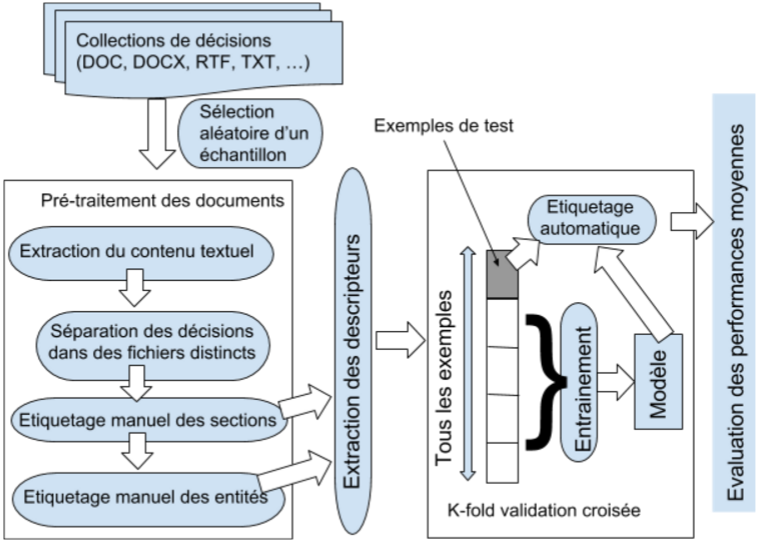
\includegraphics[scale=0.5]{archEval.PNG}
\caption{Évaluation des modèles.}
\end{figure}
\end{frame}

%\begin{frame}[c]{Approche d'application des modèles}
%\begin{figure}[t]
%\centering 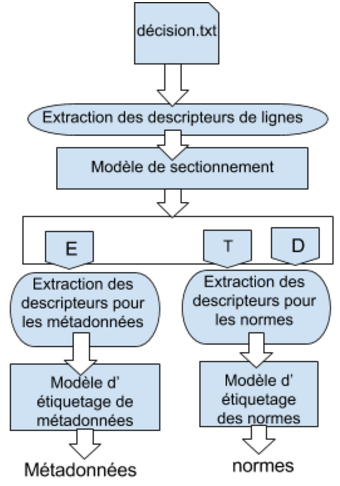
\includegraphics[scale=0.56]{archAppli.PNG}
%\caption{Application des modèles.}
%\end{figure}
%\end{frame}



\begin{frame}[c]{Conditions de tests}
\begin{itemize}
\item 505 décisions de cour d'appel annotées manuellement
\item Implémentation java (Mallet \cite{McCallum2002Mallet})
\item TreeTagger : extraction de lemmes et rôles grammaticaux
\item Implémentation de l'extraction de descripteurs (page \ref{seqTagFeatures})
\item 5-fold validation croisée
\item Précision (P), rappel (R), F1-mesure (F1):
\end{itemize}
\footnotesize
\[ P_l = \frac{\text{nombre d'éléments correctement étiquetés par le modèle avec } l}{\text{nombre d'éléments  étiquetés par le modèle avec } l} \]

\[ R_l = \frac{\text{nombre d'éléments correctement étiquetés par le modèle avec } l}{\text{nombre d'éléments manuellement étiquetés avec } l} \]

\[ F1_l = 2 \times \frac{P_l \times R_l }{P_l + R_l} \]
avec $l$=label
\end{frame}


\begin{frame}[c]{Evaluation de la détection des sections}
\begin{table}[!htb]
\footnotesize
\centering
\begin{tabular}{|c|c|c|c|c|c|c|c|c|c|}
\hline
 & \multicolumn{3}{c|}{HMM} & \multicolumn{3}{c|}{CRF-} & \multicolumn{3}{c|}{CRF+} \\
\hline
\textit{labels} & P & R & F1  & P & R & F1 & P & R & F1 \\
\hline
E (Entete)& 84.2 & 91.8 & 87.8  & 93.8 & 85.4 & 89.3 & 99.3 & 99.6 & 99.5 \\
\hline
T (Corps)& 88.4 & 63.9 & 74.1  & 86.3 & 98.2 & 91.8 & 99.8 & 99.5 & 99.7\\
\hline
D (Dispositif)& 15.4 & 47.0 & 23.0  & 100.0 & 8.5 & 15.6 & 98.0 & 100.0 & 98.9 \\
\hline
\textit{Moyenne} & 62.7 & 67.6 & 67.6  & 93.3 & 64.0 & 64.0 & 99.7 & 99.8 & 99.8  \\
\hline
\end{tabular}
\caption{Précision (P), rappel (R), F1-mesure (F1) au niveau des lignes ($\%$).}
\label{prf-zoning}
\end{table}
\end{frame}

\begin{frame}[c]{Evaluation de la détection des entités}
\begin{table}[!htb]
\footnotesize
\centering
\begin{tabular}{|c|c|c|c|c|c|c|c|c|c|}
\hline
 & \multicolumn{3}{c|}{HMM}  & \multicolumn{3}{c|}{CRF-}  & \multicolumn{3}{c|}{CRF+} \\
\hline
\textit{labels} & P & R & F1 & P & R & F1 & P & R & F1 \\
\hline
 \multicolumn{10}{|c|}{\textit{\textit{Section Entête (E)}}} \\
\hline
 AP & 35.3 &  14.1 & 20.1  & 64.9 & 48.8 & 55.6 & 92.0 & 86.7 & 89.3 \\
\hline
 AV & 83.8 &  98.3 & 90.5  & 96.4 & 97.5 & 96.9 & 97.6 & 98.1 & 97.9 \\
 \hline
 DT & 70.9 & 72.6 & 71.7  & 94.4 & 86.8 & 90.4 & 98.8 & 97.7 & 98.2 \\
 \hline
FM & 87.6 &  93.7 & 90.5  & 98.8 & 98.4 & 98.6 & 98.9 & 99.3 & 99.1 \\
 \hline
FT &  88.8 & 59.8 & 71.3  & 94.2 & 92.3 & 93.3 & 97.1 & 95.5 & 96.3 \\
 \hline
IM  & 53.1 & 57.4 & 55.1  & 67.2 & 64.6 & 65.8 &  89.3 & 88.1 & 88.7  \\
 \hline
 \textcolor{red}{IV} & - & 2.2 & - & 25.9 & 26.5 & 26.2 & 67.3 & 41.4 & \textcolor{red}{46.4} \\
 \hline
JG  & 68.0 & 85.7 & 75.7  & 96.2 & 95.7 & 96.0 & 98.1 & 97.7 & 97.9 \\
 \hline
JR  & 75.8 & 99.5 & 86.0  & 98.6 & 99.4 & 99.0 & 99.3 & 99.4 & 99.4 \\
 \hline
RG  &  - & 0  & - & 83.7 & 46.1 & 59.4 & 98.6 & 97.4 & 98.0 \\
\hline
VL & 93.1 & 27.9 & 42.6  & 98.2 & 98.4 & 98.3 & 99.0 & 99.0 & 99.0 \\
\hline
 \multicolumn{10}{|c|}{\textit{\textit{Sections inférieures (T \& D )}}} \\
 \hline
NO & 92.9 & 90.9 & 91.9 & 96.0 & 93.8 & 94.9 & 97.9 & 96.5 & 97.2\\
\hline
\end{tabular}
\caption{Précision (P), rappel (R), F1-mesure (F1) au niveau des mots ($\%$).}\label{prf-entity}
\end{table}
\end{frame}

%-=-=-=-=-=-=-=-=-=-=-=-=-=-=-=-=-=-=-=-=-=-=-=-=
%
%	Section: Classification des décisions par utilisation d’une approche semi-supervisée 
%
%-=-=-=-=-=-=-=-=-=-=-=-=-=-=-=-=-=-=-=-=-=-=-=-=
\section{Classification des décisions}

\begin{frame}{Origine: Extraction des informations sur les demandes}
\begin{block}{Informations pertinentes à extraire}
\begin{itemize}
\item \textbf{Position de la partie}: Intimé
\item \textbf{Catégorie de demande}: Dommages-intérêts pour procédure abusive
\begin{itemize}
\item \textbf{Objet}: Dommages-intérêts
\item \textbf{Fondement}: Articles 1382 code civil et 32-1 code de procédure civile
\end{itemize}
\item \textbf{Quantum demandé}: 20 000 euros
\item \textbf{Résultat} : Rejet
\item \textbf{Quantum accordé} : 0 euros
\end{itemize}
\end{block}
\end{frame}

\begin{frame}{Expression plus ou moins explicite}
\begin{exampleblock}{Expression de demande (explicite / implicite?)}
La société A. conclut à la confirmation du jugement entrepris sauf à
former appel incident sur la disposition du jugement l'ayant déboutée de sa
demande de \textbf{dommages intérêts pour abus de procédure} et elle demande à la cour de
condamner l'appelante à lui payer la somme de \textbf{20 000 euros} à titre de dommages
intérêts ...

%- \textbf{la} condamner à payer une somme de \textbf{283 589 euros} à titre de {\bf dommages et intérêts pour concurrence déloyale},

...
\end{exampleblock}

\begin{alertblock}{Expression implicite de resultat}
La cour, ... 

\textbf{Confirme la décision entreprise en toutes ses dispositions},
\end{alertblock}
\end{frame}

\begin{frame}{Extraire les demandes suivants leur catégorie}

\begin{block}{Exemples de catégorie de demande}

\begin{itemize}
\item dommages et intérêts pour procédure abusive,
\item dommages et intérêts pour concurrence déloyale,
\item dommages et intérêts pour trouble de voisinage, 
\item prestation compensatoire,
\item torts exclusifs,
\item droit de visite,
\item etc.

\end{itemize}
\end{block}

\end{frame}

\begin{frame}{Approche basée sur la catégorisation des décisions}

\begin{block}{Définition d'une classe de décision}
Soit $C$ une catégorie de demande et $D$ une décision,

s'il existe dans $D$ une demande $d$ de catégorie $C$, alors $C$ est une classe de $D$
\end{block}

\begin{alertblock}{}
\begin{itemize}
\item une décision comprend plusieurs demandes de catégories variées
\item toutes les catégories ne sont pas connues d'avance
\end{itemize}
\end{alertblock}
\end{frame}

\begin{frame}{Catégorisation semi-supervisée des décisions}
\begin{figure}
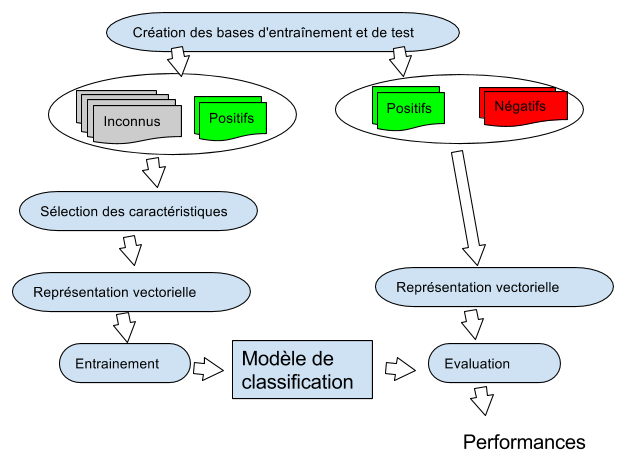
\includegraphics[scale=0.6]{archi-classif.png}
\caption{Approche d'expérimentation de la classification}
\end{figure}
\end{frame}

\begin{frame}{Création d'une base d'apprentissage}
\begin{figure}
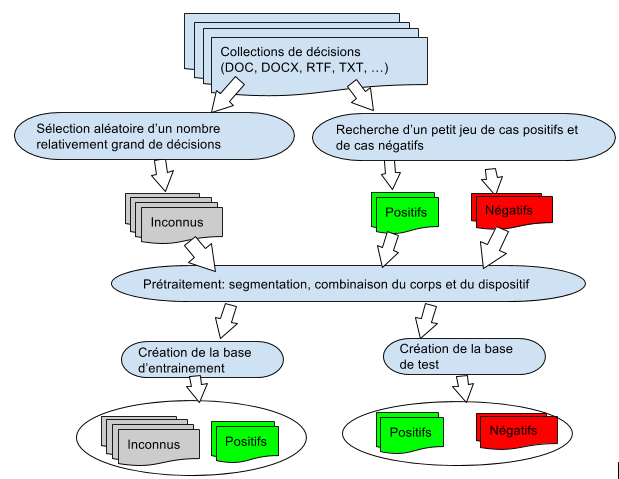
\includegraphics[scale=0.6]{createDataset-classif.png}
\caption{Etapes de création du jeu d'apprentissage}
\end{figure}
\end{frame}

\begin{frame}{Conditions d'évaluation de la catégorisation des décisions}

\begin{itemize}
\item Représentation vectorielle: {\small \[ poids(w*, t) = poids_{local}(w*, t) * poids_{global}(w*) * facteur_{normalisation}\]}
\item Évaluation de différentes configurations:
\begin{itemize}
\item dimensions des vecteurs : 2, 10, ..., 250, ...
\item méthodes de sélection de termes discriminants (p. \ref{notations} \& \ref{featuresSelectors}): $\chi^2, \Delta_{DF}, Marascuilo, NGL, GSS $  ...
\item méthodes de classification: SVM, arbre de décision, KNN, naïf bayésien (avec Weka\cite{Eibe2016Weka})
\item méthodes de pondération locale (p. \ref{localWeights}) : TF, LogTF, ATF, TP
\end{itemize}
\item environ 2000 cas inconnus, 
\item dommages-intérêts pour abus de procédure : entrainement 152 positifs, test 39 positifs + 157 négatifs
\item prestation compensatoire : entrainement 100 positifs, test 100 positifs + 100 négatifs
\item ...
\end{itemize}
\end{frame}

\begin{frame}{Mesures d'évaluation}
\scriptsize
\[ P_C = \frac{\text{nombre de décisions test correctement classées par le modèle dans } C}{\text{nombre de décisions test effectivement dans } C} \]
\[ R_C = \frac{\text{nombre de décisions test correctement classées par le modèle dans } C}{\text{nombre de décisions test effectivement dans } C} \]
\[ F1_C = 2 \times \frac{P_C \times R_C }{P_C + R_C} \]
avec $C$ = une classe de décision

\end{frame}

\begin{frame}{Premières évaluation de la classification des décisions}
\scriptsize
Est-ce l'effet de la méthode de :
\begin{itemize}
\item constitution des exemples d'apprentissage/test
\item sélection de caractéristiques
\end{itemize}
\begin{figure}
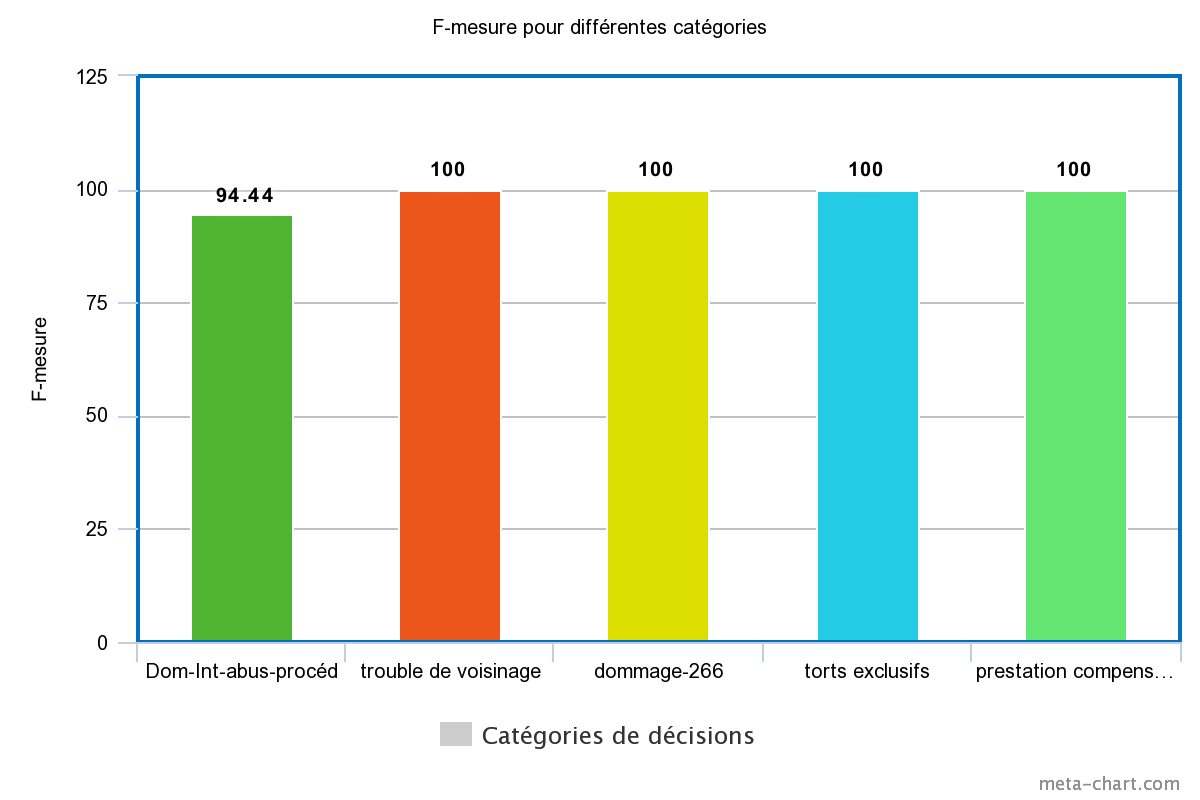
\includegraphics[width=0.8\textwidth]{f-mesure-classif.png}
\caption{Performance actuelles de classification}
\end{figure}
\end{frame}

%-=-=-=-=-=-=-=-=-=-=-=-=-=-=-=-=-=-=-=-=-=-=-=-=
%
%	Section: Coliee 2017
%
%-=-=-=-=-=-=-=-=-=-=-=-=-=-=-=-=-=-=-=-=-=-=-=-=
\section{Recherche d'information}
\begin{frame}{Problématique de Question-Réponse}
\scriptsize
\begin{alertblock}{Situation concrete}
mon mari demande le divorce, 

nous avons un prêt en commun qui finance une maison construite sur mon terrain (donation).

Je veux bien reprendre le prêt à mon nom au moment du divorce car il ne veut plus payer cette maison, mais il me réclame tout ce qu'il a payé durant notre mariage :prêt+travaux. \textbf{\large en a t'il le droit?}

j'estime ne rien lui devoir ce qui a été fait est un héritage pour nos enfants. Ce qui est sur mon terrain m'appartient je pense.

en vous remerciant

\textit{\tiny Source: \url{http://www.documentissime.fr/questions-droit/question-46724-emprunt-et-divorce.html}}
\end{alertblock}


\begin{block}{Recherche des affaires/décisions \og \textit{similaires} \fg{}}
\begin{itemize}
\item catégorie de demandes
\item éléments factuels
\end{itemize}
\end{block}

\end{frame}
\begin{frame}{Similarité avec le challenge COLIEE 2017}
\scriptsize
\begin{alertblock}{Requete: une situation abstraite}
There is a limitation period on pursuance of warranty if there is restriction due to superficies on the subject matter, but there is no restriction on pursuance of warranty if the seller's rights were revoked due to execution of the mortgage. 
\end{alertblock}

\begin{exampleblock}{1. Quels articles permettent de juger cette situation?}
\textbf{Article 566} (1)In cases where the subject matter of the sale ...

\textbf{Article 567}(1)If the buyer loses his/her ownership of ...
\end{exampleblock}

\begin{exampleblock}{2. Est-ce une situation en accord avec les articles?}
Oui
\end{exampleblock}
\textit{\tiny Source: \url{http://webdocs.cs.ualberta.ca/~miyoung2/COLIEE2017/}}
\end{frame}

\begin{frame}{Recherche des articles}
%\scriptsize
Utilisation d'une méthode d'estimation de la "pertinence" $w(A,Q)$ d'un texte $A$ pour une requête $Q$ (ex. BM25)

\centering 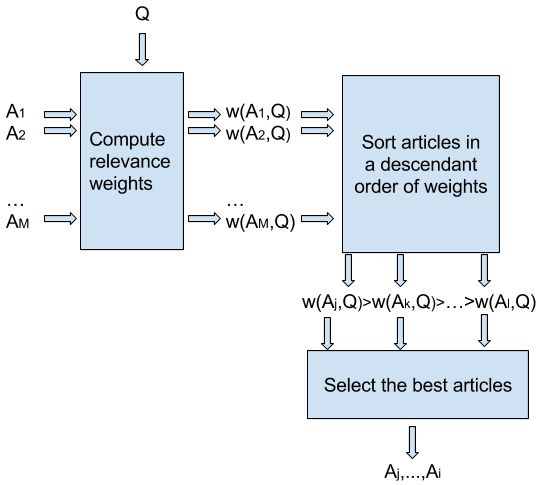
\includegraphics[scale=0.5]{coliee-bm25.png}
\end{frame}

%-=-=-=-=-=-=-=-=-=-=-=-=-=-=-=-=-=-=-=-=-=-=-=-=
%
%	Section: Conclusion
%
%-=-=-=-=-=-=-=-=-=-=-=-=-=-=-=-=-=-=-=-=-=-=-=-=
\section{Conclusion}

\begin{frame}{Etat d'avancement:}
\begin{itemize}
\item Détection d'entités et de sections
\begin{itemize}
\item Performances encourageantes du CRF
\item Difficultés:
\begin{itemize}
\item Annotation manuelle d'un jeu suffisant d'exemples
\item Identification de bons descripteurs 
\end{itemize}
\item Limite de l'approche:
\begin{itemize}
\item descripteurs définis manuellement (portabilité des modèles)
\end{itemize}
\end{itemize}
\item Classification des décisions:
\begin{itemize}
\item à partir d'un petit nombre de décisions d'une catégorie, il est possible de retrouver les termes caractéristiques des catégories
\end{itemize}
\end{itemize}

\end{frame}

\begin{frame}[c]{Perspectives}
\begin{itemize}
\item Détection d'entités et de sections
\begin{itemize}
\item Amélioration des performances (ex.  plus d'exemples d'entêtes avec les intervenants)
\item Apprendre automatiquement une représentation (ex. deep learning)
\item Résolution et désambiguïsation des entités

\begin{center}
\textit{article {\bf 700} = article {\bf 700} du \textcolor{red}{Code de Procédure Civile}}
\end{center}

\item Etendre l'étude à d'autres juridictions
\end{itemize}
\item Extraction de demandes:
\begin{itemize}
\item Comment exploiter les termes clés d'une catégorie pour retrouver les demandes dans les décisions?
\end{itemize}
\end{itemize}
\end{frame}

\begin{frame}{Le projet global}
Objectif: Mettre sur pied des moyens efficaces :
\begin{itemize}
\item de structuration d'un corpus exhaustif des décisions (en général)

\item d'analyses dans ce corpus
\end{itemize}

Défis divers à relever en informatique:
\begin{itemize}
\item extraction d'information
\item représentation des connaissances
%\item apprentissage automatique
\item recherche d'information
\end{itemize}
\end{frame}

%%-=-=-=-=-=-=-=-=-=-=-=-=-=-=-=-=-=-=-=-=-=-=-=-=
%%
%%	Questions
%%
%%-=-=-=-=-=-=-=-=-=-=-=-=-=-=-=-=-=-=-=-=-=-=-=-=
\section{Questions?}
%-=-=-=-=-=-=-=-=-=-=-=-=-=-=-=-=-=-=-=-=-=-=-=-=
%	References:
%-=-=-=-=-=-=-=-=-=-=-=-=-=-=-=-=-=-=-=-=-=-=-=-=
\begin{frame}[t,allowframebreaks]{References}
\tiny
\bibliographystyle{apalike}
\bibliography{references}	
\end{frame}

\begin{frame}[c]{Descripteurs de lignes pour le sectionnement}
\label{seqTagFeatures}
\begin{enumerate}
\item HMM : numéro de ligne
\item CRF : 
\begin{itemize}
\item numéro de ligne
\item toute la ligne
\item les 3 premiers termes
\item le nombre de termes
\item 1er terme des lignes suivantes et précédentes
\item ...
\end{itemize}
\end{enumerate}
\end{frame}

\begin{frame}[c]{Descripteurs de mots pour les entités}
Pour les entités de l'entête:
\begin{enumerate}
\item HMM : le mot
\item CRF : 
\begin{itemize}
\item mot
\item lemme
\item rôle grammatical
\item commence-t-il par une lettre majuscule ?
\item le texte contient-il la chaine « intervenant » ?
\item ...
\end{itemize}
\end{enumerate}
\end{frame}

\begin{frame}[c]{Descripteurs de mots pour les entités}
Pour les normes:
\begin{enumerate}
\item HMM : le mot
\item CRF : 
\begin{itemize}
\item mot
\item lemme
\item rôle grammatical
\item le mot est-il un terme clé des normes ? (\textit{article, code, loi,
contrat, règlement, convention, décret})
\item noms ou adjectifs voisins
\item ...
\end{itemize}
\end{enumerate}
\end{frame}

\begin{frame}{Sélection des caractéristiques d'une catégorie de décisions}
\label{notations}
\scriptsize 
\textbf{Notations (Pour le corpus d'entrainement)} \\
$w$ : un terme \\
$t$: un texte \\
$L_w$ : longueur de $w$ (nommbre de mots) \\
$c$ : la classe cible ou positive (catégorie de demande)\\
$\overline{c}$ : la classe complémentaire ou négative (inconnue) \\
$N_{c}$ et $N_{\overline{c}}$ : resp. nombre de textes de $c$ et de $\overline{c}$\\
$N_{w,c}$ : nombre de textes de $c$ contenant $w$ \\
$N$ : nombre total de textes dans le corpus ($N = N_{c} + N_{\overline{c}}$)\\
$DF_c$ : proportion de textes du corpus appartenant à $c$ ($\p(c)$ : probabilité qu'un texte pris au hasard soit de la classe $c$ )\\
%$TF_{w \vert c}$ : fréquence d'observations $w$ dans $c$ (en prenant un terme au hasard parmi les (occurences de) termes de $c$) \\
$DF_w$: proportion de documents du corpus contenant $w$ ("Document frequency")\\
$DF_{w \vert c}$ : proportion de documents de $c$ contenant $w$ \\
$DF_{c \vert w}$ : proportion de documents contenant $w$ qui appartiennent à $c$ ($\p(c \vert w)$=)\\
$Occ_{w,t}$: nombre d'occurrences de $w$ dans $t$ \\
$Occ_t$: somme des nombres d'occurrences des termes dans $t$ \\
$TF_{w,t}$: fréquence d'observation de $w$ dans le texte $t$ \\
$SI_{w}$ : score d'importance de $w$ pour $c$

\end{frame}

\begin{frame}{Sélection des caractéristiques d'une catégorie de décisions}
\label{featuresSelectors}
\scriptsize 

\[\Delta_{DF}(w,c) = DF_{w,c} - DF_{w,\overline{c}}\]

\[\chi^2(w,c) = \frac{N ((N_{w,c} N_{\overline{w},\overline{c}}) - (N_{w,\overline{c}} N_{\overline{w},c}))^2}{N_w N_{\overline{w}} N_c N_{\overline{c}}}\]

\[ngl(w,c) = \frac{\sqrt{N} ((N_{w,c} N_{\overline{w},\overline{c}}) - (N_{w,\overline{c}} N_{\overline{w},c}))}{\sqrt{N_w N_{\overline{w}} N_c N_{\overline{c}}}}\]

\[gss(w,c) = (N_{w,c} N_{\overline{w},\overline{c}}) -  (N_{w,\overline{c}} N_{\overline{w},c})\]


Marascuilo:
\[M(w,c) = \frac{(N_{w,c} - N_{w}N_c/N)^2 + (N_{w,\overline{c}} - N_{w}N_{\overline{c}}/N)^2 + (N_{\overline{w},c} - N_{c}N_{\overline{w}}/N)^2 + (N_{\overline{w},\overline{c}} - N_{\overline{w}}N_{\overline{c}}/N)^2 }{N}\]

\end{frame}

\begin{frame}{Méthode de pondération locale}
\label{localWeights}
\scriptsize 

\begin{table}[!htb]
\centering
\begin{tabular}{|p{0.4\textwidth} p{0.4\textwidth}|}
\hline
\textbf{Méthode} & \textbf{Formule}  \\ \hline
 &  \\
Fréquence de $w*$  & $TF_{w*,t} = \frac{Occ_{w*,t}}{\sum\limits_{w_i \in W} Occ_{w_i,t}}$ \\ \hline
 &  \\ 
Présence de $w*$  & $TP_{w*,t} = \left\lbrace \begin{array}{cl}
1 & \text{si }TF_{w*,t} > 0 \\
0 & sinon
\end{array} \right.$ \\ \hline
 &  \\ 
Fréquence augmentée de $w*$ & $ATF_{w*,t} = k + (1-k) \frac{TF_{w*,t}}{\max\limits_{w_i \in W} TF_{w_i,t}}$  \\ \hline
 &  \\ 
Logarithme de la fréquence de $w*$ & $LogTF_{w*,t} = \log{(TF_{w*,t}+1)}$  \\ \hline
\end{tabular}
\caption{Méthodes de pondération locale} \label{PoidsLocal}
\end{table}
\end{frame}

\end{document}
